\documentclass{article}
\usepackage{amsmath, sfmath, multicol, tkz-euclide, array, enumerate, tcolorbox, tabularray}
\renewcommand{\familydefault}{\sfdefault}
\setlength{\parindent}{0cm}
\pagestyle{empty}
\usepackage[left=1in, top=0.5in, right=1in, bottom=0.5in]{geometry}
\tikzset{>=stealth}
\tcbset{colback=white}

\newcounter{example}[section]
\newenvironment{example}[1][]{\refstepcounter{example}\par\medskip
   {\color{red}\textbf{Example~\theexample. #1}}}{\medskip}

\begin{document}

\section*{Similarity in Right Triangles}

\begin{tcolorbox}[colframe=orange!70!white, coltitle=black, title=\textbf{Today I Can}]
\begin{enumerate}
    \item Find and use relationships in similar right triangles.
\end{enumerate}
\end{tcolorbox}
\smallskip

\begin{tcolorbox}[colframe=black!20!white, opacitybacktitle=0.1, coltitle=black, title=\textbf{Altitudes in Right Triangles}]
An altitude drawn from the right angle of a right triangle creates 3 similar triangles. \newline 

\begin{minipage}{0.4\textwidth}
\begin{itemize}
    \item $\triangle ABC \sim \triangle CBD \sim \triangle ACD$
\end{itemize}
\end{minipage}
\begin{minipage}{0.5\textwidth}
    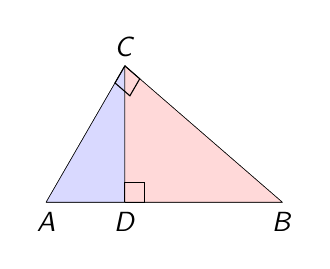
\begin{tikzpicture}
    \tkzDefPoints{0/0/A, 3/0/B, 1/0/D}
    \tkzDefLine[orthogonal = through D](A,B)
    \tkzGetPoint{E}
    \tkzDefShiftPoint[A](60:0.5){F}
    \tkzInterLL(A,F)(E,D) 
    \tkzGetPoint{C}
    \tkzDrawPolygon(A,B,C)
    \tkzDrawSegment(C,D)
    \tkzLabelPoints[below](A,D,B)
    \tkzLabelPoints[above](C)
    \tkzDrawPolygon[fill=blue!15](A,D,C)
    \tkzDrawPolygon[fill=red!15](B,D,C)
    \tkzMarkRightAngles(B,D,C A,C,B)
    \end{tikzpicture}
\end{minipage}
\begin{center}
    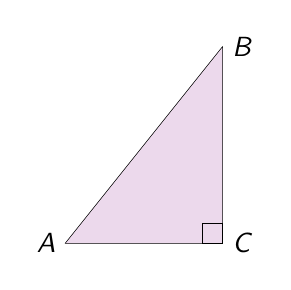
\begin{tikzpicture}
    \tkzDefPoints{0/0/A, 2/0/C, 2/2.5/B}
    \tkzDrawPolygon[fill=violet!15](A,B,C)
    \tkzMarkRightAngle(B,C,A)
    \tkzLabelPoints[left](A)
    \tkzLabelPoints[right](B,C)
    \end{tikzpicture}
\hspace{0.2in}
    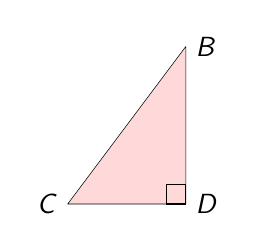
\begin{tikzpicture}
    \tkzDefPoints{0.5/0/C, 2/0/D, 2/2/B}
    \tkzDrawPolygon[fill=red!15](D,B,C)
    \tkzMarkRightAngle(C,D,B)
    \tkzLabelPoints[right](D,B)
    \tkzLabelPoints[left](C)
    \end{tikzpicture}
\hspace{0.2in}
    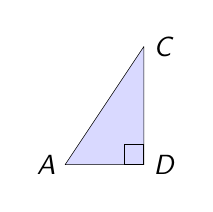
\begin{tikzpicture}
    \tkzDefPoints{0/0/A, 1/0/D, 1/1.5/C}
    \tkzDrawPolygon[fill=blue!15](A,D,C)
    \tkzLabelPoints[left](A)
    \tkzLabelPoints[right](D,C)
    \tkzMarkRightAngle(A,D,C)
    \end{tikzpicture}
\end{center}
\end{tcolorbox}
\smallskip 

\begin{example}
 What similarity statement can you write relating the three triangles in each diagram?
\begin{multicols}{2}
\begin{enumerate}[(a)]
    \item \mbox{} \newline 
    \item \mbox{} \newline 
\end{enumerate}
\end{multicols}
\begin{minipage}{0.5\textwidth}
    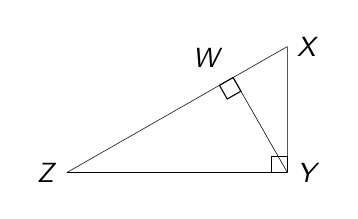
\begin{tikzpicture}[scale=0.8]
    \tkzDefPoints{0/0/Z, 3.5/0/Y, 3.5/2/X}
    \tkzDrawPolygon(X,Y,Z)
    \tkzLabelPoints[left](Z)
    \tkzLabelPoints[right](Y,X)
    \tkzMarkRightAngle(Z,Y,X)
    \tkzDefLine[orthogonal=through Y](X,Z)
    \tkzGetPoint{A}
    \tkzInterLL(Y,A)(X,Z)
    \tkzGetPoint{W}
    \tkzDrawSegment(W,Y)
    \tkzLabelPoints[above left](W)
    \tkzMarkRightAngle(Y,W,Z)
    \end{tikzpicture}
\end{minipage}
\begin{minipage}{0.4\textwidth}
    \begin{tikzpicture}[scale=0.8]
    \tkzDefPoints{0/0/S, -1.5/0/Q, 2.5/0/R, 0/-2/P}
    \tkzDrawPolygon(Q,P,R)
    \tkzDrawSegment(S,P)
    \tkzLabelPoints[above](Q,S,R)
    \tkzLabelPoints[below](P)
    \tkzMarkRightAngles(R,S,P Q,P,R)
    \end{tikzpicture}
\end{minipage}
\end{example}

\vfill 

\begin{tcolorbox}[colframe=black!20!white, opacitybacktitle=0.1, coltitle=black, title=\textbf{Geometric Mean}]
The \textbf{geometric mean}, $x$, of two positive numbers $a \text{ and } b$ is the solution of 
\[
\frac{a}{x} = \frac{x}{b}
\]
\end{tcolorbox}
\smallskip 

\begin{example}
Find the geometric mean of each pair of numbers.
\begin{multicols}{2}
\begin{enumerate}[(a)]
    \item 6 and 15
    \item 4 and 18
\end{enumerate}
\end{multicols}
\end{example}

\vspace{0.5in}

\newpage 

\begin{tcolorbox}[colframe=black!20!white, opacitybacktitle=0.1, coltitle=black, title=\textbf{Altitude as a Geometric Mean}]
An altitude drawn from the right angle of a right triangle is the geometric mean of the 2 segments it creates on the hypotenuse. \newline 

\begin{minipage}{0.4\textwidth}
\begin{itemize}
    \item $\frac{a}{y} = \frac{y}{b}$
\end{itemize}
\end{minipage}
\begin{minipage}{0.4\textwidth}
    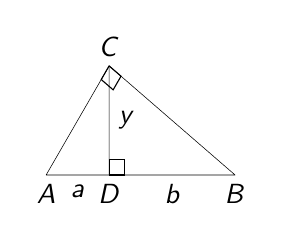
\begin{tikzpicture}[scale=0.8]
    \tkzDefPoints{0/0/A, 3/0/B, 1/0/D}
    \tkzDefLine[orthogonal = through D](A,B)
    \tkzGetPoint{E}
    \tkzDefShiftPoint[A](60:0.5){F}
    \tkzInterLL(A,F)(E,D) 
    \tkzGetPoint{C}
    \tkzDrawPolygon(A,B,C)
    \tkzDrawSegment(C,D)
    \tkzLabelPoints[below](A,D,B)
    \tkzLabelPoints[above](C)
    \tkzMarkRightAngles(B,D,C A,C,B)
    \tkzLabelSegment[right](C,D){$y$}
    \tkzLabelSegment[below](A,D){$a$}
    \tkzLabelSegment[below](D,B){$b$}
    \end{tikzpicture}
\end{minipage}
\end{tcolorbox}
\smallskip 

\begin{tcolorbox}[colframe=black!20!white, opacitybacktitle=0.1, coltitle=black, title=\textbf{Leg as a Geometric Mean}]
If an altitude is drawn from the right angle of a right triangle, then a leg is the geometric mean of the large triangle's hypotenuse and the segment on the large hypotenuse adjacent to the leg. \newline 

\begin{minipage}{0.4\textwidth}
\begin{itemize}
    \item $\frac{a}{x} = \frac{x}{b}$
\end{itemize}
\end{minipage}
\begin{minipage}{0.4\textwidth}
    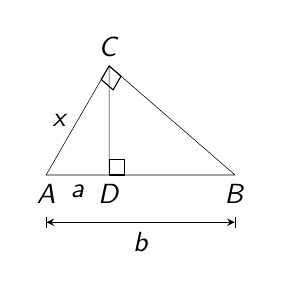
\begin{tikzpicture}[scale=0.8]
    \tkzDefPoints{0/0/A, 3/0/B, 1/0/D}
    \tkzDefLine[orthogonal = through D](A,B)
    \tkzGetPoint{E}
    \tkzDefShiftPoint[A](60:0.5){F}
    \tkzInterLL(A,F)(E,D) 
    \tkzGetPoint{C}
    \tkzDrawPolygon(A,B,C)
    \tkzDrawSegment(C,D)
    \tkzLabelPoints[below](A,D,B)
    \tkzLabelPoints[above](C)
    \tkzMarkRightAngles(B,D,C A,C,B)
    \tkzLabelSegment[left](C,A){$x$}
    \tkzLabelSegment[below](A,D){$a$}
    \tkzDefPoints{0/-0.75/W, 3/-0.75/V}
    \tkzDrawSegment[|<->|, >=stealth](W,V)
    \tkzLabelSegment[below](V,W){$b$}
    \end{tikzpicture}
\end{minipage}
\end{tcolorbox}
\smallskip

\begin{example}
Find the values of $x$ and $y$ in each.
\begin{multicols}{2}
\begin{enumerate}[(a)]
    \item \mbox{} \newline 
    \item \mbox{} \newline 
\end{enumerate}
\end{multicols}
\begin{minipage}{0.5\textwidth}
    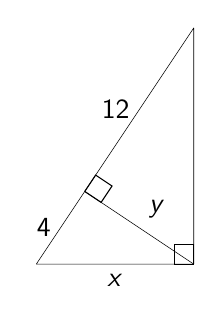
\begin{tikzpicture}
    \tkzDefPoints{0/0/A, 2/0/B, 2/3/C}
    \tkzDrawPolygon(A,B,C)
    \tkzDefLine[orthogonal=through B](A,C)
    \tkzGetPoint{D}
    \tkzInterLL(B,D)(A,C)
    \tkzGetPoint{E}
    \tkzDrawSegment(B,E)
    \tkzMarkRightAngles(A,B,C B,E,C)
    \tkzLabelSegment[below](A,B){$x$}
    \tkzLabelSegment[left](A,E){4}
    \tkzLabelSegment[left](E,C){12}
    \tkzLabelSegment[above right](B,E){$y$}
    \end{tikzpicture}
\end{minipage}
\begin{minipage}{0.4\textwidth}
    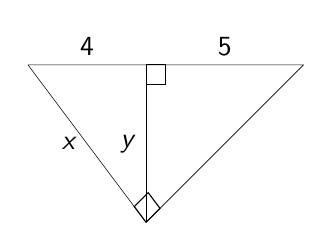
\begin{tikzpicture}
    \tkzDefPoints{0/0/S, -1.5/0/Q, 2/0/R, 0/-2/P}
    \tkzDrawPolygon(Q,P,R)
    \tkzDrawSegment(S,P)
    \tkzMarkRightAngles(R,S,P Q,P,R)
    \tkzLabelSegment[above](Q,S){4}
    \tkzLabelSegment[above](R,S){5}
    \tkzLabelSegment[left](P,Q){$x$}
    \tkzLabelSegment[left](P,S){$y$}
    \end{tikzpicture}
\end{minipage}
\end{example}

\end{document}
